% example of how to use template

% set the template of document
\documentclass[natbib]{muthesis}
\usepackage{graphicx}
\usepackage{url}
\usepackage{float}
\usepackage{subfig}
\usepackage{etoolbox}
\usepackage{mathtools,amsmath}
\usepackage{physics}
\usepackage{empheq}
\usepackage{esdiff}
\restylefloat{table}
\restylefloat{figure}
\usepackage{caption}
\bibliographystyle{plain} % if you are using bibtex
\graphicspath{ {./images/} }

% create new command for convenience
% \newcommand{\beq}{\begin{equation}}
% \newcommand{\eeq}{\end{equation}}
% \newcommand{\bfig}{\begin{figure}}
% \newcommand{\efig}{\end{figure}}
% \newcommand{\bfa}{\left\{\begin{array}}
% \newcommand{\efa}{\end{array}\right.}
% \renewcommand{\arraystretch}{1.5}

% set number of candidate (from 1 - 3) and advisor (from 1 - 2)
\noofcandidate{1}
\noofadvisor{1}

% information for front page
\title{Automatic Subtitle Generator}
\candidate{Aphisit Areechitsakul}

\degree{B.Sc.}
\subject{Computer Science}
\submissionyear{2020}

% information for page i (advisors)
\candidatetitle{}
\majoradvisor{Dr.Sunsern Cheamanunkul}
\majoradvisorsubject{Computer Science}

% information for page ii (exam committee)
\submissiondate{8th April 2020}

% Advisor
\advisor{Dr.Sunsern Cheamanunkul}

% Program Director
\programdirector{Dr. Kritya Bunchongchit}
% Division Chair
\chair{Assoc. Prof. Dr. Pakorn Bovonsombat}

% information for page iv (ABSTRACT)

\candidatenumber{5880685 ICCS/B}

%\longsubject
\keywords{speech recognition, word error rate}

% information for biography

% For first candidate
\dateofbirth{8th November 1997}
\placeofbirth{Samut Sakhon , Thailand}
\firstdegree{IGCSE}
\firstdegreemajor{Grade 11}
\firstdegreeinstitution{Traill International School}
\firstdegreeyears{2012-2014}
\years{2016-2020}
\homeaddress{51/7 moo 3 Soi Ekkachai 147 Ekkachai Road}
\homeaddressLnII{T. Bangnamjeud A.Muang}
\homeaddressLnIII{Samut Sakhon, 74000, Thailand}
\email{bright40081@gmail.com}

\begin{document}

  \maketitle

  \acknowledgements{
	I would like to express my thanks of gratitude to my advisor Dr.Sunsern Cheamanunkul, and other professors at MUIC who given me the knowledge during my college years on campus. I also would like to thank my family and friends for their support and encouragement throughout my whole journey.
  }

  \abstract{
  	Automatic subtitle generator is a system for generating video subtitles automatically. The typical process involves extracting speech data from the video, transcribing the speech into text, and reconstruct the subtitles using the transcribed text along with the timing information. In this thesis, we design and implement an online automatic subtitle generator by leveraging online speech recognition services and open-source software libraries. Our implementation consists of a VueJS-based frontend and a Python-based backend. To generate a video with subtitles, one just needs to upload a video and choose a speech recognition engine from our list. Additionally, we evaluate the accuracy of different speech recognition engines. We found that YouTube speech recognition service has the lowest word error rate. Lastly, we also explore the idea of gender recognition through speech for subtitle annotation.
  }

  % Table of content
  \linespacing{1.2}
  \tableofcontents

  \linespacing{1.77}

% \cite{name}
% ------ Chapter 1 -------
  \chapter{Introduction}
  \section{Motivation}
  Video is one of the popular media that people can easily access and watch it for various purposes, such as education and entertainment. Nevertheless, many of us cannot fully understand the content of the video due to the language barrier. As such, subtitle plays an important role to help us understand more about the part of the content that we missed. It also helps us to feel familiar with the accent and pronunciation, which allows us to improve our language skills better. Moreover, having subtitles gives the opportunity for deaf people enjoy videos. Deaf people normally watch the videos with either sign languages or subtitles, but not all videos come with them, especially lecturing and recording video types.
  
  %---change to 2 point---
  \section{Objective}
  There are two main objectives of this project. The first one is to implement the web service for automatic subtitle generator by making use of the existing speech recognition services and open-sources, including Amazon Transcribe, CMUSphinx, DeepSpeech and Google Web Speech, and the second goal is to evaluate and discuss the performance of each speech recognition system.
  
  \section{Timeline}
  The gantt chart below shows the duration of each step during development.
    \begin{figure}[H]
  	\centering
  	\captionsetup{justification=centering}
  	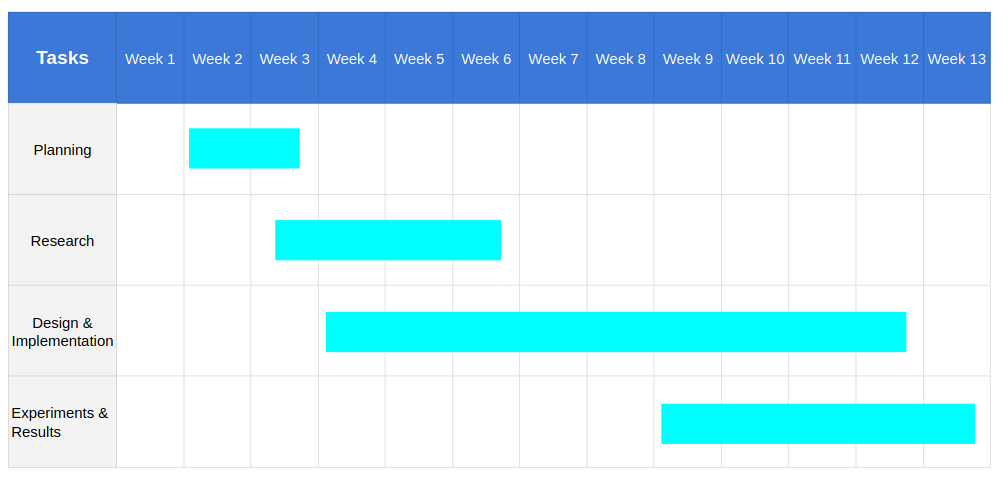
\includegraphics[width=0.9\linewidth]{images/gantt-chart}
  	\caption{Gantt chart}
  	\label{fig:gantt-chart}
  \end{figure}
  
  % ------ Chapter 2 -------
  \chapter{Literature Review}
  
  \section{Overview of Existing Automatic Subtitle Generator}
  Many online platforms that related to videos now provide a feature for generating the subtitle of video. YouTube, an online video sharing platform, Facebook, a social media platform, and Veed, an online video editor service, are one of those examples that allow us to use this feature for free. However, the generated subtitles are not perfect, the service provider also come up with the subtitle editor so that users can fix it on spot.
  
  In order to build up the automatic subtitle generator(ASG) service, automatic speech recognition is required to recognize the speeches in video.
  \section{Overview of Automatic Speech Recognition}
  
  \begin{figure}[H]
  	\centering
  	\captionsetup{justification=centering}
  	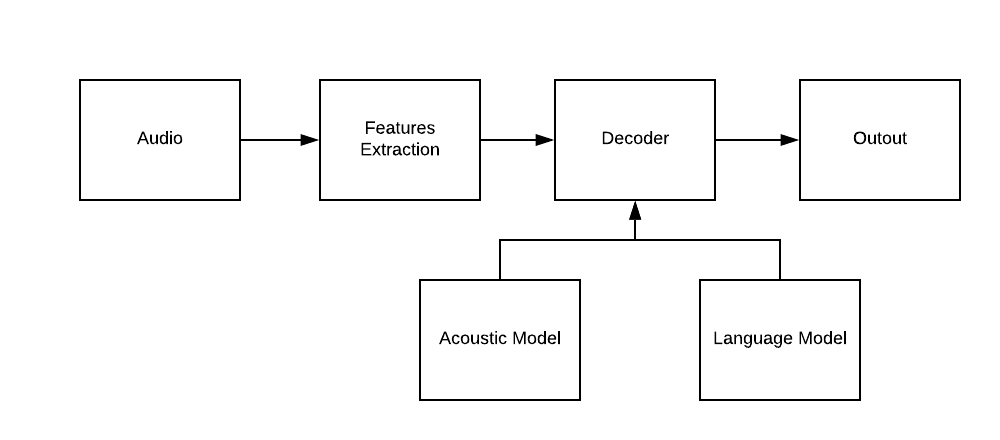
\includegraphics{images/traditional-asr}
  	\caption{Traditional ASR pipeline}
  	\label{fig:traditional-asr}
  \end{figure}
  Automatic Speech Recognition(ASR) is a technology that allows the computer to identify human spoken words and convert them into the digital text. The main components in ASR are acoustic and language models.
  Figure 2.1 illustrates the flow of traditional automatic speech recognition for transcribing.
  Firstly, It takes in the audio wave as an input and extract its features in preprocessing step. During the decoding part, the system uses acoustic model to recognize the phonetics from the data representation and decode them through the language model to produce the proper text. 
  
  Originally, the acoustic model is trained by using Gaussian Mixture Model(GMM) based Hidden Markov Model(HMM) system, but as technology become more developed, Deep Neural Network(DNN) replaced GMM with a higher accuracy.\cite{Shivakumar_2019} Nowadays, there are many ways of training methods and configurations, and each speech recognition engine has their own ways. In this paper, there are four ASR systems introduced
  \subsection{Amazon Transcribe}
  Amazon Transcribe is one of the well known automatic subtitle speech recognition services provided by Amazon. It is an online service that allows users to convert the speech into text from either video or audio at a rate of \$0.0004 per second. The technique that could possibly be used to train the acoustic model is semi-supervised learning. The type of model is HMM-LSTM hybrid.\cite{parthasarathi2019lessons}
  \subsection{CMUSphinx / Pocketsphinx}
  Pocketsphinx is one of the speech recognition engines developed by Carnegie Mellon University. It is a lightweight speech recognition for handheld but also usable on desktop. The acoustic model of Pocketsphinx either trains through continuous or semi-continuous HMM while the language model is either modeled through  a statistical language model or finite state grammar.\cite{PocketSphinx} 
  
  \subsection{DeepSpeech}
  DeepSpeech is an open source project that aims to create the Speech-To-Text engine. The machine learning methods in training the models are based from the Baidu DeepSpeech research paper. According to the paper, acoustic model is trained by using the Recurrent Neural Network (RNN) with no Long-short-term-memory(LSTM), and language model is trained by using N-Gram\cite{hannun2014deep}.
  The version and model that used in this project are 0.6.1 and pre-trained model that trained on American English with the data from LibraSpeech and achieved an 7.5\% word error rate. 
  \subsection{Google Web Speech API}
  Google Web Speech API or Google Speech Recognition is an online paid service provided by Google at a cost of \$0.006 per 15 seconds. The python library used in this project provides the default API key, but it comes with the limit of the amount that users can request per day. The methods that used to train the model possibly is Listen, Attend and Spell(LAS) with an unidirectional LSTM.\cite{46687} It is a deep neural network that combining different kinds of models, including acoustic model, language model and pronunciation model.
% ------ Chapter 3 -------
 \chapter{Design And Implementation}
 The basic idea for automatic subtitle generator(ASG) is simple. Imagine that users have videos that want to generate the subtitle. They upload it to the ASG service to get the results in either subtitle files or overlayed videos.
 
 \begin{figure}[H]
 	\centering
 	\captionsetup{justification=centering}
 	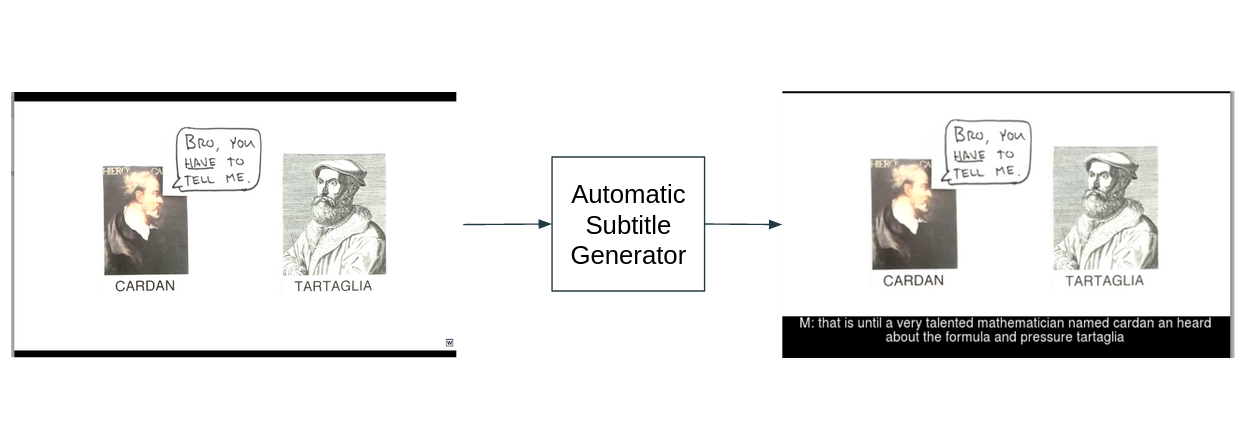
\includegraphics[width=1.0\linewidth]{images/overview-asg}
 	\caption{Oveview of the Automatic subtitle generator}
 	\label{fig:overview-asg}
 \end{figure}
 \section{Overall Architecture}
 %images
 
 \begin{figure}[H]
 	\centering
 	\captionsetup{justification=centering}
 	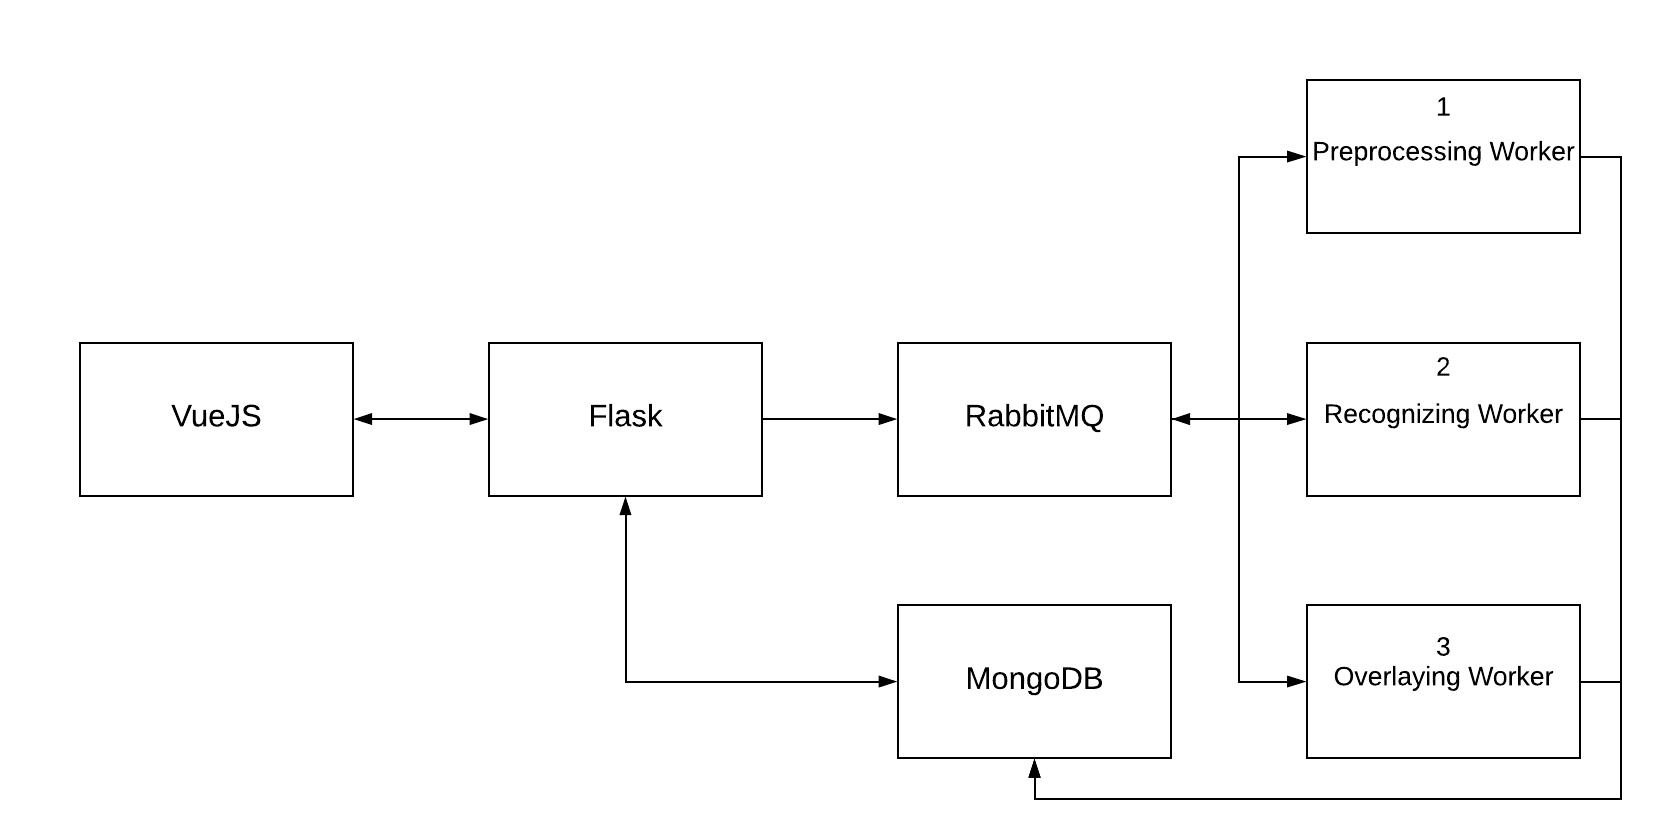
\includegraphics[width=1.0\linewidth]{images/overall-architecture}
 	\caption{Overall Architecture of the system}
 	\label{fig:overall-architecture}
 \end{figure}
 
 Figure 3.2 illustrates the flow of the entire framework that implemented on the service. First, users upload the video through the frontend, VueJS. After the backend server gets the data from API, it stores the video into local storage and updates the video status in the database, MongoDB. Later it sends the jobs to celery workers through the message-broker, RabbitMQ. The worker that firstly receive the job is the preprocessing worker and followed by recognizing worker and overlaying workers.
 
 \section{Frontend}
 VueJS is used to build up the web pages. There are only two pages, which are the upload video page and the video information page.
 On the upload page, users have to choose the video that they want to generate subtitles and select the recognizer before uploading the video. Otherwise, the error message will appear on the page.
 %image
 \begin{figure}[H]
	\centering
	\captionsetup{justification=centering}
	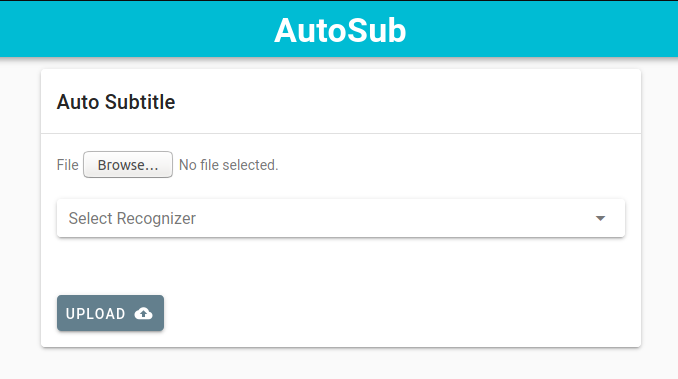
\includegraphics[width=0.8\linewidth]{images/main}
	\caption{Frontend main page}
	\label{fig:frontend-main}
 \end{figure}

\begin{figure}[H]
\centering
\captionsetup{justification=centering}
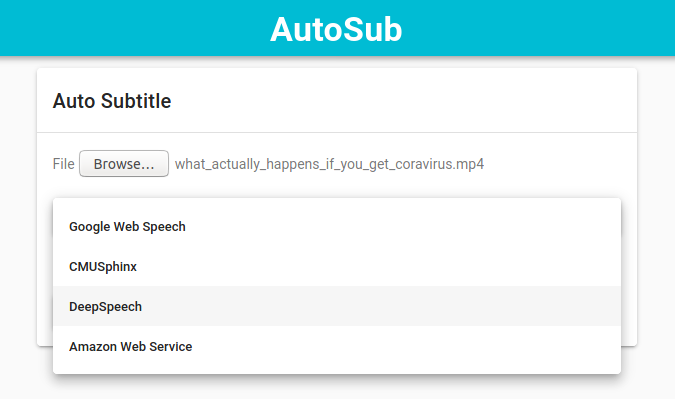
\includegraphics[width=0.8\linewidth]{images/main-with-options}
\caption{Available choices of speech recognition systems}
\label{fig:frontend-main-with-options}
\end{figure}
 
 On the video information page, it shows the video's id, filename and the status of the video. There are 5 kinds of statuses including `Video Uploaded', `Preprocessing Audio', `Recognizing Speeches', `Overlaying video with the subtitle' and `Completed'. Moreover, on this page, users are allowed to download two kinds of results, which are the generated subtitle file and overlayed video.
 %image
 \begin{figure}[H]
 	\centering
 	\captionsetup{justification=centering}
 	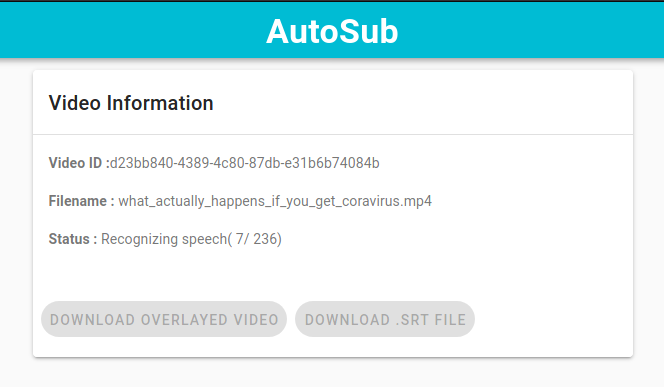
\includegraphics[width=0.8\linewidth]{images/info-recognizing}
 	\caption{The video information and status page}
 	\label{fig:frontend-info}
 \end{figure}

 \begin{figure}[H]
 	\centering
 	\captionsetup{justification=centering}
 	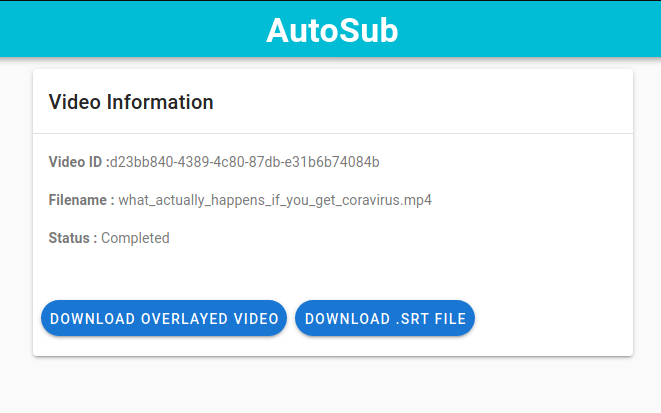
\includegraphics[width=0.8\linewidth]{images/info-completed}
 	\caption{The final look after the process is completed}
 	\label{fig:frontend-info-complete}
 \end{figure}
 
 \section{Database}
 For the database, MongoDB is selected. The design of database on this service is simple. The only data stored in the database is the information of videos. This includes of id, filename, current status of the process, total amount of detected speech regions and the current number of recognized speeches.
 
 \section{Backend}
 In the backend, Flask is used as a server to communicate between frontend and backend. There is a total of 4 APIs, which are the following.
 \begin{itemize}
 	\setlength\itemsep{0em}
 	\item \textbf{/api/upload}: an API for uploading video
 	\item \textbf{/api/get-status}: an API for getting the information of video
 	\item \textbf{/api/get-srt}: an API for downloading subtitle file
 	\item \textbf{/api/get-video}: an API for downloading overlayed video
 \end{itemize}
 
 For the backend process, Celery is used to distribute the tasks from queues to the workers while having RabbitMQ as a message-broker. 
 
 Celery is an asynchronous task queue based on distributed messages.\cite{CeleryProj}
 RabbitMQ is a lightweight open source message broker that supports multiple messaging protocols.\cite{Rabbit}
 
 \section{Preprocessing Worker}
 The first job for this worker is to update the video status in the database to preprocessing status.
 In the preprocessing worker, the audio is processed by the steps in subsections. 
 However, unlike other speech recognition systems, Amazon Transcribe is an online paid service. It has different ways to process the audio, and our job is to upload the original video to the Amazon S3 bucket and create a transcribed job. After the whole process is done, the worker will update the status in the database.
 
 \subsection{Processioning Audio}
 There are some steps required in this process. Since the input of the system is video, the first step in the process is to extract the audio from the video. After that, we need to convert the audio channels from stereo to mono by averaging the signal of left and right channels, and the last requirement is to resample the audio to 16000Hz.
 Filtering audio is one additional process to reduce the noise and non-speech regions of audio. In order to do this, a band-pass filter is applied to filter out audio wave at human range fundamental frequency, which is around 85 to 255Hz with some extra padding\cite{nagaraja2019voiploc}.
 
 \subsection{Voice Activity Detection}
 After preprocessing the audio, the worker will detect the speech regions inside audio by using voice activation detection(VAD). Voice activity detection is a technique that uses for distinguishing speech segments from background noise, and there are many ways to do it. The algorithm in this project is based on calculating the energy threshold. Firstly, the process takes the sampling windows of the audio data and converts the values of sampling windows into energies using root-mean-square(RMS). Root-mean-square is the formula to calculate the average energy of the amplitudes. After getting an array of energies, we decided and calculate the cutoff percentile of energy to decide whether the windows are silence and speech. The last part of this algorithm is to loop over the sampling windows and find the speech segments by comparing the energy with the threshold.\cite{VADEnergybase}
 \begin{figure}[H]
 	\centering
 	\captionsetup{justification=centering}
 	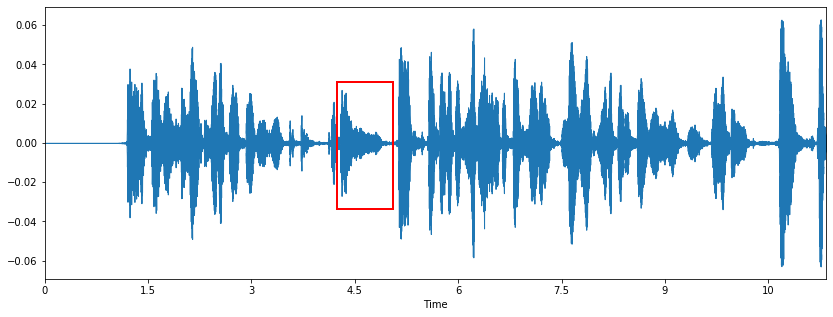
\includegraphics[width=0.9\linewidth]{images/vad}
 	\caption{Illustration of Voice Activity Detection}
 	\label{fig:vad}
 \end{figure}
 
 
 The drawback of this algorithm is that detected segments might be the background noise and music instead.
 
 After calculating the speech regions of the audio, we split the audio file into smaller chunks according to the audio segments.
 
 \section{Recognizing Worker}
 At the beginning of this process, the worker updates the video status to recognizing status. The main job of this worker is to recognize speeches from the audio chunks using the selected speech recognition system. Apart from the Amazon Transcribe, the other three systems have the same flow. First, the worker reads the data from audio chunks and lets the speech recognition recognize the audio, and every time that speech is recognized, the worker will update the recognizing process status in the database. However, some audio chunks are not speeches or recognizable resulting in errors, such as unknown value error and empty string. Thus, we need to reconstruct the sentences again base on the text and timing gap of each phrase.
 
 For the Amazon Transcribe, after createing the transcribed job, the worker will wait until the job is complete and retrieve the JSON result that consists of words, punctuation and timestamps. Then, the worker constructs the phrases based on them.
 
 The last step left in this worker is to generate the subtitle file by using the result we get.
 
 \section{Overlaying Worker}
 At the beginning of the process, the worker updates the video status to overlaying. The package that used to overlay the video is moviepy, a python module for video editing. The first step that the worker does is to load up the generated subtitle file from recognizing worker and the original video data. Then, moviepy read each phrase and timestamp of the subtitle and overlay on the original video. Overlaying video required a lot of memory usage, so rendering video with lower quality is an extra option. Lastly, the worker updates the video status to the complete stage, which allows users to download the video.
 
 % ------ Chapter 4 -------
 \chapter{Experiments and Results}
 
 To set up the experiments for ASG system, we collected the videos from YouTube, and manually extract human and YouTube generated transcript from the video as the ground truths for calculating the word error rate. The below table shows the list of videos used in these experiments.
 
 \begin{center}
 	\scalebox{0.9}{
 		\begin{tabular}{ |c|c|c| } 
 			\hline
 			No. & Video Name & Type \\ 
 			\hline
 			0 & Conversation Between Two Friends In English Speaking(Dialogue 1)\cite{ConversationBTW2Friends} & Dialogue \\
 			1 & Conversation Between Two Friends In English Speaking(Dialogue 2)\cite{ConversationBTW2Friends} & Dialogue \\
 			2 & Imaginary Numbers Are Real [Part 2: A Little History]\cite{ImaginaryNumber} & Math \\
 			3 & Joker Final Trailer (2019)\cite{JokerTrailer} & Entertainment \\
 			4 & Spider-Man: Into the Spider-Verse Trailer & Entertainment\\
 			5 & Teaching Methods for Inspiring the Students of the Future(4 minutes)\cite{TeachingMethod} & Public Speaking \\
 			6 & The Most Beautiful Equation in Math\cite{MathEq} & Math \\
 			7 & Think Fast, Talk Smart: Communication Techniques(4 minutes)\cite{TFTS} & Public Speaking \\
 			8 & What Actually Happens If You Get Coronavirus?\cite{Coronavirus} & Science\\
 			9 & What makes a good teacher great?(4 minutes)\cite{GoodTeacher} & Public Speaking\\
 			
 			\hline
 	\end{tabular}}
 \end{center}


 A screenshot shown below comes from the video list called ``What Actually Happens If You Get Coronavirus?''. This video will be used as the main example for automatic subtitle generator  
 \begin{figure}[H]
 	\centering
 	\captionsetup{justification=centering}
 	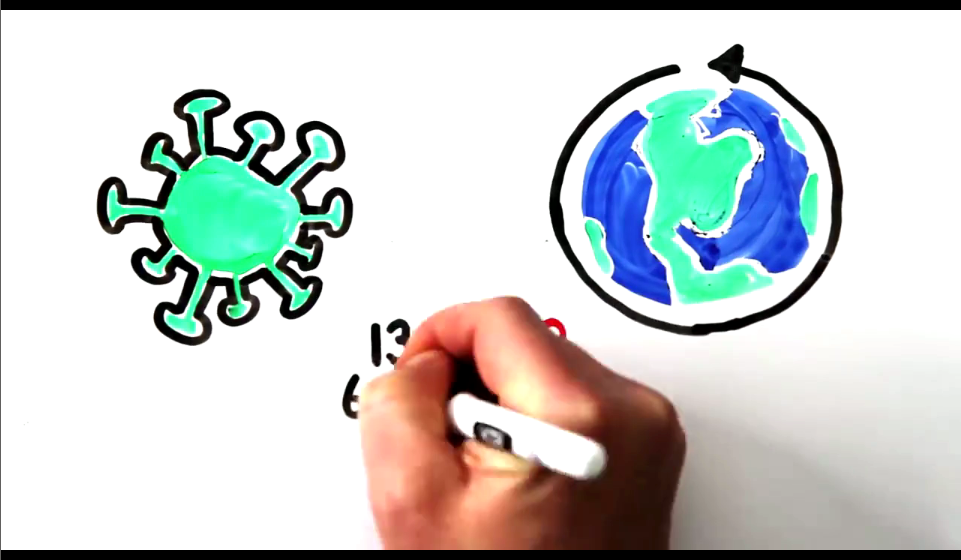
\includegraphics[width=0.7\linewidth]{images/example-video-original}
 	\caption{A screenshot from the example video}
 	\label{fig:example-vidoe-original}
 \end{figure}

 
 \section{Result of Automatic Subtitle Generator}
 
 \begin{figure}[H]
 	\begin{minipage}{0.5\textwidth}
 		\centering
 		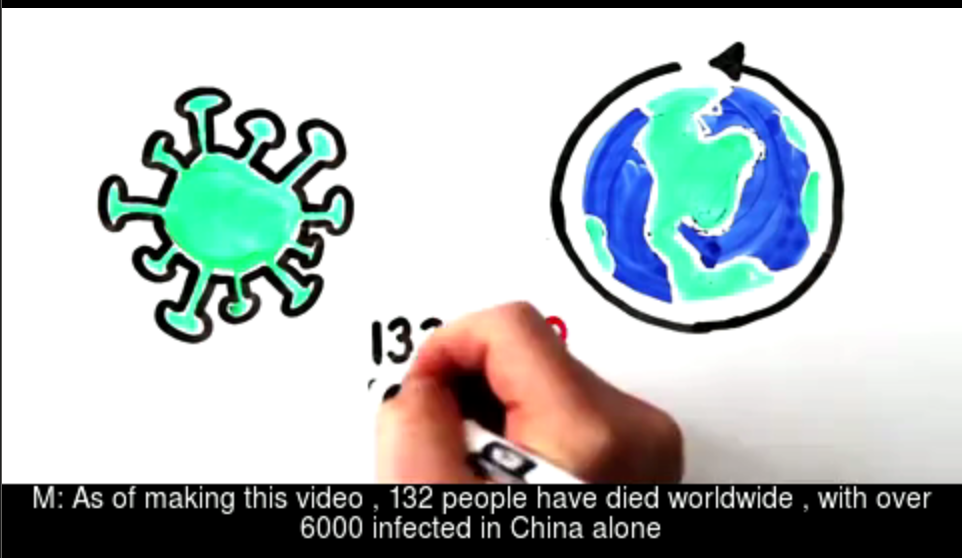
\includegraphics[width=0.9\textwidth]{images/example-video-aws} 
 		\captionof{figure}{Amazon Transcribe}
 		\label{fig:example-video-aws]}
 	\end{minipage}\hfill
 	\begin{minipage}{0.5\textwidth}
 		\centering
 		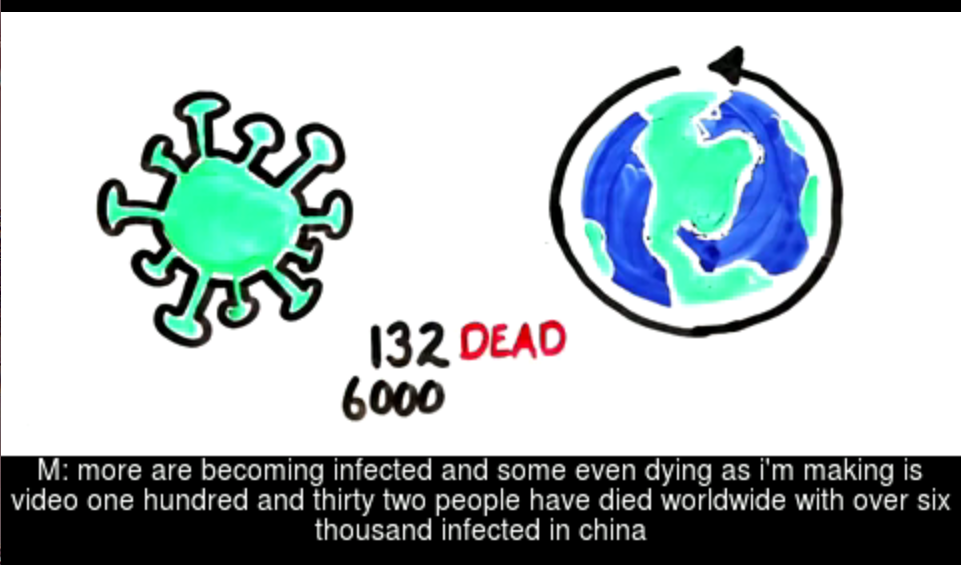
\includegraphics[width=0.9\textwidth]{images/example-video-cmusphinx} 
 		\captionof{figure}{CMUSphinx}
 		\label{fig:example-video-cmusphinx}
 	\end{minipage}
 \end{figure}
 
 \begin{figure}[H]
 	\centering
 	\begin{minipage}{0.5\textwidth}
 		\centering
 		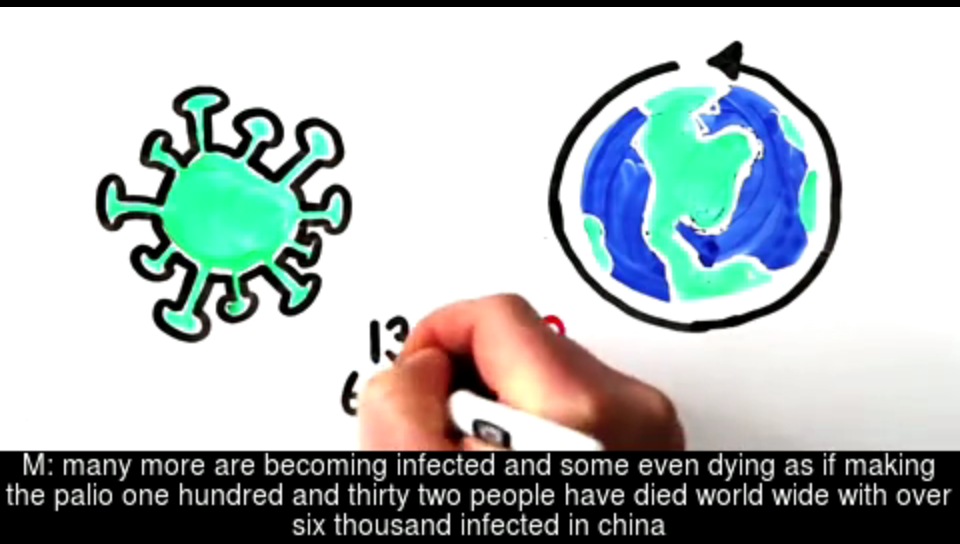
\includegraphics[width=0.9\textwidth]{images/example-video-ds} 
 		\captionof{figure}{DeepSpeech}
 		\label{fig:example-video-ds}
 	\end{minipage}\hfill
 	\begin{minipage}{0.5\textwidth}
 		\centering
 		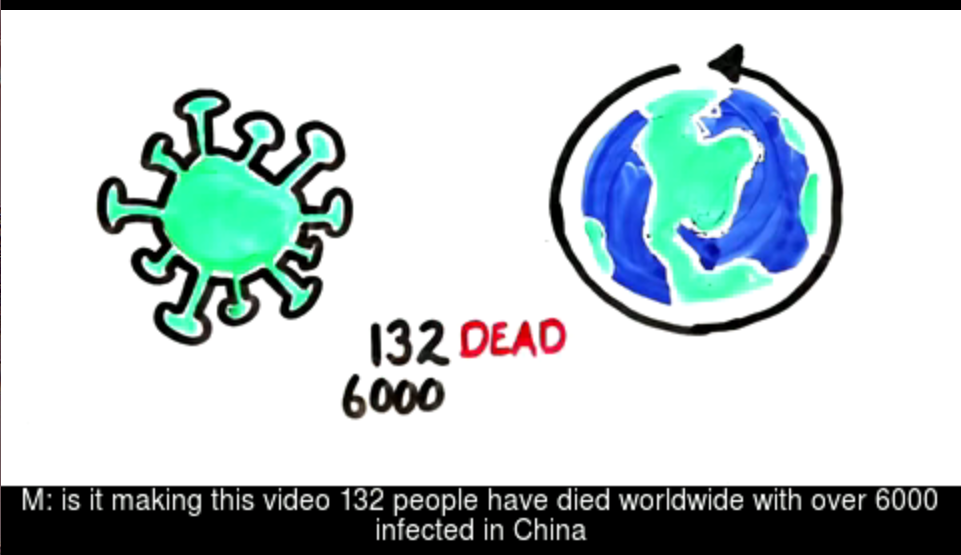
\includegraphics[width=0.9\textwidth]{images/example-video-gws} 
 		\captionof{figure}{Google Web Speech}
		\label{fig:example-video-gws}
 	\end{minipage}
 \end{figure}

  The figures above are the videos that have the subtitles generated and overlayed through the automatic subtitle generators with different speech recognition systems.
  
 \section{Accuracy Evaluation}
 
 Word error rate(WER) is a common metric that use to measure the performance of speech recognition and translation system. The lower word error rate is, the higher accuracy that the models can make. It is calculated by
 
 $$ WER = \frac{S+I+D}{N} $$
 
 S, I and D stand for substitutions, insertions and deletions, respectively. They are the number of errors that occurred in the speech recognition output. Substitutions are the text output that replaced the original text. Insertions are the extra words that speech recognition produced. Deletions are the words that were dropped from the original text. N is the total word count of the ground truth text.
 
 Before using the word error rate, there are still some considerations that need to be mentioned. First, the word error rate excludes the punctuation in the calculation. Second, word error doesn't tell the source of errors that occurred. Third, although the word error rate can tell the performance of a speech recognition system, it cannot entirely tell the usability of the system.
 
 
 The table and box-plot on the figures below tell the word error rates that calculated from testing videos.
 \begin{figure}[H]
 	\centering
 	\captionsetup{justification=centering}
 	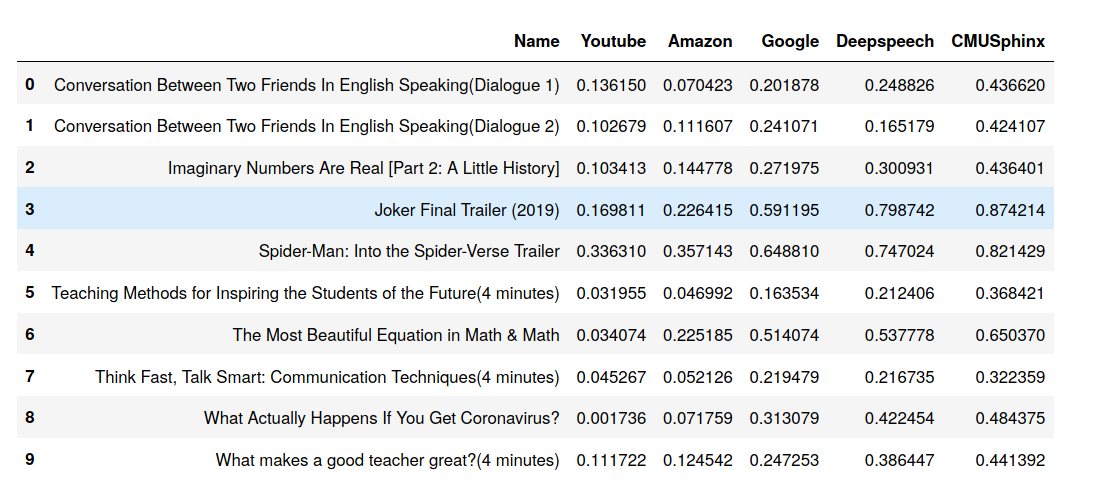
\includegraphics[width=1\linewidth]{images/wer-table}
 	\caption{A WER table of testing videos}
 	\label{fig:wer-table}
 \end{figure} 
 
  \begin{center}
  	\begin{tabular}{ |c|c| } 
  		\hline
  		Speech Recognition System & Avg. WER.  \\ 
  		\hline
  		YouTube & 10.7\%\\ 
  		Amazon Transcribe & 14.3\% \\
  		Google Web Speech & 34.1\% \\
  		DeepSpeech & 40.4\% \\
  		CMUSphinx & 52.6\% \\
  		\hline
  	\end{tabular}
  \end{center}

 \begin{figure}[H]
 	\centering
 	\captionsetup{justification=centering}
 	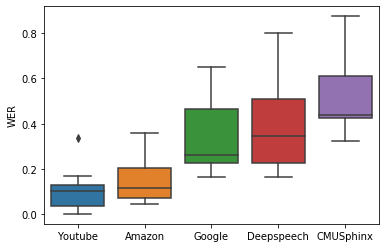
\includegraphics[width=0.7\linewidth]{images/boxplot}
 	\caption{A WER box-plot of testing videos}
 	\label{fig:wer-boxplot}
 \end{figure}

 
 According to the table and box-plot, YouTube has the lowest word error rate compared to others. The second is by Amazon Transcribe and then followed by Google Web Speech, DeepSpeech and CMUSphinx, respectively. 
 \section{Discussion}
 
 This section is dedicated to discussing the reasons why the performance of the speech recognition system is low and will be categorized into four parts below
 \subsection{Names and Acronyms}

 From the observations on text output, there are times that the speech recognition systems unable to recognize the words. The table below shows the examples of this error 
 \begin{center}
 	\begin{tabular}{ |c|c|c| } 
 		\hline
 		Speech Recognition System & Names & Acronym  \\ 
 		\hline
 		Ground truth & coronavirus & DNA or RNA\\
 		YouTube & coronavirus & DNA or RNA\\ 
 		Amazon Transcribe & corona virus & DNA or RNA\\
 		Google Web Speech & coronavirus & DNA or are\\
 		DeepSpeech & corona virus, cronies, crown virus &Diana or are\\
 		CMUSphinx & roto virus, throw the virus	& DNA of war are nay\\
 		\hline
 	\end{tabular}
 \end{center}
 
 As shown in the table, DeepSpeech and CMUSphinx are clearly two of the speech recognition system that failed to recognize the word and produce sound-alike word instead. However, it is also because that the words ``Coronavirus'', ``DNA'' and ``RNA'' are the technical terms that people rarely talk about, so the pre-trained models are likely to focus more on the common speeches. Unlike the other two, Youtube, Amazon Transcribe and Google Web Speech are large groups of providers and their target come from various groups of users, so their models are more adaptable and keep updating.
 
 \subsection{Number}
 As mentioned earlier, the word error rate cannot entirely describe the usability of the system, the number is one of the examples. The table below shows examples of this issue.
 \begin{center}
 	\begin{tabular}{ |c|c|c| } 
 		\hline
 		Speech Recognition System & Example 1 \\ 
 		\hline
 		Ground truth & 132 people have died \\
 		YouTube & 132 people have died \\ 
 		Amazon Transcribe & 132 people have died \\
 		Google Web Speech & 132 people have died \\
 		DeepSpeech & one hundred and thirty two people have died \\
 		CMUSphinx & one hundred and thirty two people have died \\
 		\hline
 	\end{tabular}
 \end{center}
 \begin{center}
 	\begin{tabular}{ |c|c|c| } 
 		\hline
 		Speech Recognition System & Example 2 \\ 
 		\hline
 		Ground truth & \$1,\$2 and \$5\\
 		YouTube & \$1,\$2 and \$5\\ 
 		Amazon Transcribe & \$1.2 dollars and \$5\\
 		Google Web Speech & \$1,\$2 + \$5\\
 		DeepSpeech & one dollar two dollars and five dollars\\
 		CMUSphinx & one dollar dollars and five dollars\\
 		\hline
 	\end{tabular}
 \end{center}
 From the table, we can see that the outputs are understandable. However, if we look into the word error rate calculation, the number and symbol could be considered as errors instead.
 
 In example 1, ground truth is ``132 people have died''. The numerical character in text ``132'' can also be read as ``one hundred and thirty two'', so from the users' perspective, they can understand both. However, in terms of word error rate, this kind of result can affect its last value. For example, in the calculation, ``132'' is considered as one word, but on the other hand, ``one hundred and thirty two'' is considered as five error words. If we use ``132'' as the ground truth, the word error will be 5. This situation also applied to the example 2, where ``\$1'' is considered as one word while ``one dollar'' is considered as two words
 
 In terms of usability, both kinds are fine, but if the task requirement is the numerical character, YouTube, Amazon Transcribe and Google Web Speech are the good choices. Even so, there are times that the engines recognize them as words, which also depend on the structure of sentences.
 
 
 \subsection{Accent, Pronunciation and Noise}
 Accent, pronunciation and noise are some of the main reasons that cause the system unable to recognize the words or sentences. If the model is not trained for the particular accent and pronunciation, there is a high chance that the accuracy of the speech recognition will be low and effect the word error rate.
 
 \begin{center}
 	\scalebox{0.9}{
 	\begin{tabular}{ |c|c| } 
 		\hline
 		Speech Recognition System & Example  \\ 
 		\hline
 		Ground truth & But what we will be looking at is how the corona virus actually.. \\
 		YouTube & But what we will be looking at is how the corona virus actually..\\ 
 		Amazon Transcribe & But what we will be looking at is how the corona virus actually \\
 		Google Web Speech & coronavirus Act \\
 		DeepSpeech & by that we will be looking at is how the crown a virus act actually \\
 		CMUSphinx & we will be looking at is how the krown virus\\
 		\hline
 	\end{tabular}}
 \end{center}

 From the table above, the ground truth is ``But what we will be looking at''. This phrase comes from the video called ``What Actually Happens If You Get Coronavirus?''\cite{Coronavirus} at 33 seconds of video. There are two speakers in videos, and this phrase is the transition between them. For this example, we will focus on the word, ``But what''. At the start of this phrase, the speaker speaks this word at a fast pace which causes some speech recognition engine unable to recognize the text. For example, DeepSpeech listen to it as ``by that'', while Google Web Speech API and CMUDSphinx unable to transcribe the beginning of sentence
 
 To give another example, the table below shows the WER that calculated from the video on YouTube called Joker Final Trailer. As the video is a movie trailer, the video has a lot of noise and background music as well as the accent and pronunciation that different from a normal video. 

 \begin{center}
 	\begin{tabular}{ |c|c| } 
 		\hline
 		Speech Recognition System & WER(\%)  \\ 
 		\hline
 		YouTube & $16.98\%$  \\ 
 		Amazon Transcribe & $22.64\%$  \\
 		Google Web Speech & $59.12\%$ \\
 		DeepSpeech & $79.87\%$\\
 		CMUSphinx & $87.42\%$ \\
 		\hline
 	\end{tabular}
 \end{center}

 As shown in the table, the good speech recognition engine like YouTube also produced the high word error rate and followed by Amazon Transcribe, Google Web Speech, DeepSpeech and CMUSphinx, respectively.
 
 \subsection{Systems Evalaution}
 In this subsection, we will give the pros and cons of that found in each speech recognition engine. 
 
 
 From the observations, it could be concluded the YouTube is the best one so far with the lowest word error rate even though sometimes it failed to transcribe, especially on entertainment video. Amazon Transcribe won in second place. It has a low word error rate and comes with punctuation, which helps us to construct new phrases easily. Another good point is that it can detect the numerical character. Google Web Speech API resulted in third place. It could detect numerical characters like Amazon Transcribe, but sometimes, it could not identify the transition or short words of audio like ``yes'', ``but'' and ``or.''
 
 
 DeepSpeech resulted in the fourth place in this competition, The main drawback is that it could not detect the name and acronym. Moreover, the pre-trained model is limit to American English, so sometimes, it could not predict other accents and pronunciation. CMUSphinx achieved the highest word error rate, and most of the cases, CMUSphinx predict the words that have the sound alike, but this doesn't mean that it cannot be used. The pre-trained model provided by CMUSphinx can do better in the videos that used lots of common words.
 
 Despite the fact of these results, the evaluation could differ depending on the different configurations and settings.
 
 \chapter{Gender Recognition}
 First to mention that the gender recognition system for this project is an additional feature and incomplete, and there are many improvements need to be done.
 
 Gender recognition by voice is a machine learning technique that is utilized to determine the gender of speakers by processing audio signals.
 
 
 \section{Dataset}
 We rely on the voice data provided by Kory Becker with the total amount of 3,168 records of male and female voices, and the data is preprocessed with 21 features.\cite{Dataset}
 \begin{itemize}
 	  \setlength\itemsep{0em}
 \item \textbf{meanfreq}: mean frequency (in kHz)
 \item \textbf{sd}: standard deviation of frequency
 \item \textbf{median}: median frequency (in kHz)
 \item \textbf{Q25}: first quantile (in kHz)
 \item \textbf{Q75}: third quantile (in kHz)
 \item \textbf{IQR}: interquantile range (in kHz)
 \item \textbf{skew}: skewness (see note in specprop description)
 \item \textbf{kurt}: kurtosis (see note in specprop description)
 \item \textbf{sp.ent}: spectral entropy
 \item \textbf{sfm}: spectral flatness
 \item \textbf{mode}: mode frequency
 \item \textbf{centroid}: frequency centroid (see specprop)
 \item \textbf{peakf}: peak frequency (frequency with highest energy)
 \item \textbf{meanfun}: average of fundamental frequency measured across acoustic signal
 \item \textbf{minfun}: minimum fundamental frequency measured across acoustic signal
 \item \textbf{maxfun}: maximum fundamental frequency measured across acoustic signal
 \item \textbf{meandom}: average of dominant frequency measured across acoustic signal
 \item \textbf{mindom}: minimum of dominant frequency measured across acoustic signal
 \item \textbf{maxdom}: maximum of dominant frequency measured across acoustic signal
 \item \textbf{dfrange}: range of dominant frequency measured across acoustic signal
 \item \textbf{modindx}: modulation index. Calculated as the accumulated absolute difference between adjacent measurements of fundamental frequencies divided by the frequency range
 label: male or female
 \end{itemize}
 \section{Model Training and Results}
 The gender recognition models can be trained by various techniques. However, in this paper, only some classification methods are used to train the models, including Support Vector Machine(SVM), K-Nearest Neighbor(KNN), Naive-Bayes and Random Forest.
 
 The table shown below is the evaluation of the models using k-fold cross-validation, where k is equal to 10
 \begin{center}
  \begin{tabular}{ |c|c| } 
 	\hline
 	Classification Methods& Mean Accuracy(+/ std)) \\ 
 	\hline
 	K-Nearest Neighbor & $95.83\% \pm 2.5 $\\
 	Naive-Bayes & $86.17\% \pm 7.3 $\\
 	Random Forest & $96.65\% \pm 2.5 $\\
 	Support Vector Machine & $96.81\% \pm 2.2 $\\
 	
 	\hline
  \end{tabular}
 \end{center}
 The accuracy seems to be very high. However, the models are overfitting and failed to generalize. This means that the models could not predict the gender correctly on the new data. The results are mostly gone in one way either all males or all females.
 
 \chapter{Conclusion}

 The web service implementation for automatic subtitle generator is built by using the VueJS-based frontend and Flask, python-based, backend. The overall process of the system includes three major processes, including preprocessing, recognizing and overlaying. The preprocessing process involves extracting speech data and timing information from the video. In the recognizing process, the automatic speech recognition systems are used to transcribe the speech data into text. Additionally, in this process, we reconstruct the sentences from the transcribed results and timing data before generating the new subtitle files. For the overlaying process, the python library, moviepy is used to overlay the original video with the subtitles. In order to generate the subtitles of video, users just need to upload the video and select the speech recognition system through the upload page. After uploading the video, the backend server saves the video to local storage and inserts the new data into MongoDB. Later, the server sends the tasks to workers responsible for different processes by using Celery and RabbitMQ. After the whole process is complete, the users are now allowed to download the generated video.
 
 For the automatic speech recognition systems, there are four options that users can choose, which are Amazon Transcribe, CMUSphinx, Deep Speech and Google Web Speech. From the accuracy evaluation and problem discussions between these systems with YouTube. YouTube is found to achieve the lowest word error rate with the mean around 10.7\%
 
 
  \bibliography{ref}
  \biography
  
\end{document}

